\section{Task 2: Logistic Regression}
\subsection{Subsample}
The train data set is unbalanced (1\% positive, 99\% negative). To balance the data set and reduce the training time, we subsample the negative data set to 20 passages per query and keep all positive passages. For these queries with less than 20 negative passages, we keep all negative passages. The subsampled data set has 95874 passages for 1000 queries.
\subsection{Word Embedding}
We choose Word2Vec to generate word embedding for each term in the vocabulary. The word embedding is a 100-dimensional vector. We use the pre-trained word embedding and set the window size to 5. The word embedding is trained on train and validation data set separately.
\subsection{Logistic Regression}
Logistic function:
\begin{equation}
\sigma_{\mathbf{w}}\left(\mathbf{x}_i\right)=\left(1+e^{-\mathbf{w}^{\top} \mathbf{x}_i}\right)^{-1}
\end{equation}
with weight $w$. The loss function is cross-entropy loss function $\mathcal{J}(\mathbf{w})$:
\begin{equation}
-\frac{1}{n} \sum_{i=1}^n\left[y_i \ln \left(\sigma_w\left(x_i\right)\right)+ \\
\left(1-y_i\right) \ln \left(1-\sigma_w\left(x_i\right)\right)\right]
\end{equation}
The gradient of the loss function is:
\begin{equation}
\frac{\partial \mathcal{J}(\mathbf{w})}{\partial \mathbf{w}_j} = -\frac{1}{n} \sum_{i=1}^n\left[x_{i, j}(y_i-\sigma_w\left(x_i\right)\right]
\end{equation}
We use batch stochastic gradient descent to train the model and stop our training when the validation loss does not decrease for 3 epochs. The word embedding of a query-passage pair given by two vectors with 100 dimensions. We concatenate the two vectors and add a bias term to the model and get a 201-dimensional vector.
\\\\
We initialize the weight vector with 0, set the batch size to 5000, the tolerance to 1e-8, and the maximum number of epochs to 100. To assess the effect of learning rate on our training, we vary the learning rate from 0.01 to 0.0001 and plot the training loss curve in Fig \ref{fig:lr_100}. A larger learning rate results in faster convergence and smaller train loss in the initial epoch. However, all the learning rates converge to the same loss value (0.2) after 100 epochs, except for 0.0001, which still shows no sign of convergence. To confirm convergence, we train the model with 0.0001 for 1000 epochs and present the results in Fig \ref{fig:lr_1000}. The loss converges to 0.2 within 1000 epochs.
\\\\
We decide to use a learning rate of 0.005, batch size of 5000, and epoch number of 100 for the remaining training. Table \ref{tab:lr_metrics} displays the metrics of the model on the validation set.
\\\\
We set the cutoff to 100 and apply the model to predict the relevance scores of passages for each query in the file \textsl{candidate\_passages\_top100.tsv}. We save the top 100 highest-scoring passages for each query in a file called \textsl{LR.csv}.

\begin{figure}
    \centering
    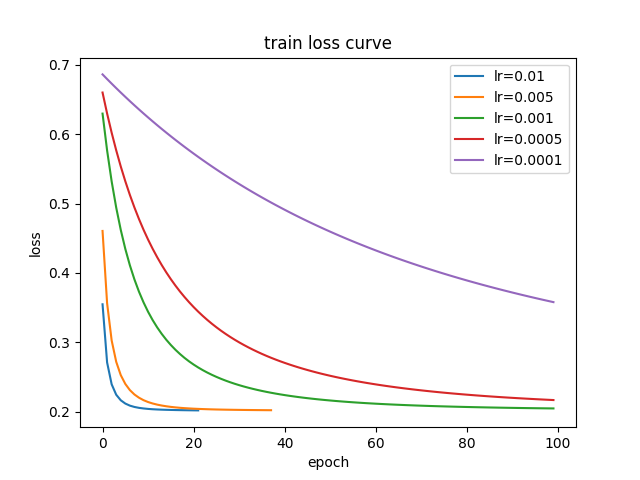
\includegraphics[width=0.5\textwidth]{aseets/epochto100.png}
    \caption{Training loss curve}
    \label{fig:lr_100}
\end{figure}
\begin{figure}
    \centering
    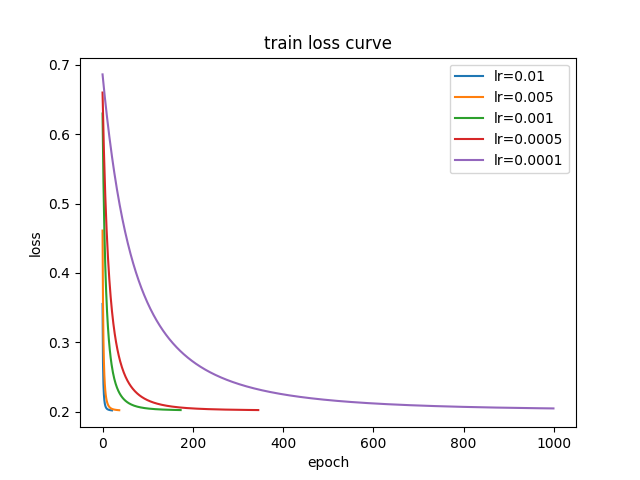
\includegraphics[width=0.5\textwidth]{aseets/epochto1000.png}
    \caption{Training loss curve}
    \label{fig:lr_1000}
\end{figure}
\begin{table}[ht]
    \centering
    \caption{Metrics of LR model}
    \label{tab:lr_metrics}
    \begin{tabular}{|c|c|c|c|}
        \hline
        LR & Cutoff & mAP & mNDCG \\
        \hline
        Top 100 & 100 & 0.0090 & 0.1254 \\
        \hline
    \end{tabular}
\end{table}